\documentclass{article}
\usepackage{tikz, comment}
\usepackage{pifont}
\usepackage{fontspec, pgfplots}
\usetikzlibrary{arrows, decorations.markings, decorations.pathreplacing}
\begin{comment}
:Title: Not defined yet
:Tags: absolute value rules;properties of equality, equation rules;equivalence properties of equality;set;proper subset
:Prob: 0.7512;0.6682;0.5893;0.5712;0.568
:Author: Prof.Hu Ji-shan, HKUST
:Slug: No name yet

Description Here.........
\end{comment}
\begin{document}\centering 

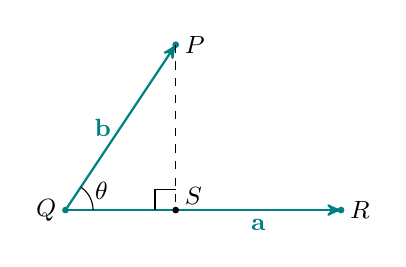
\begin{tikzpicture}[>=latex,xscale=.5*7, yscale=.5*7][font=\sf\small] 

\draw[teal, fill] (0, 0) circle(0.01)node[black, left] {$Q$};
\draw[teal, fill] (1, 0) circle(0.01)node[black, right] {$R$};
\draw[teal, fill] (0.4, 0.6) circle(0.01)node[black, right] {$P$};

\draw[teal, thick, ->, >=stealth'] (0,0)--(1, 0)
node[below, midway, pos=0.7, xshift=0, yshift=0, scale=1]{${\bf a}$};

\draw[teal, thick, ->, >=stealth'] (0,0)--(0.4, 0.6)
node[left, midway, pos=0.5, xshift=0, yshift=0, scale=1]{${\bf b}$};

\draw[dashed] (0.4, 0.6)--(0.4, 0);

\draw[] (0.325, 0)--++(0, 0.075)--++(0.075, 0);

\draw[black, fill] (0.4, 0) circle(0.01)node[black, right, yshift=5] {$S$};

\draw[samples=100, smooth, domain=0:56.3, variable=\x] 
		plot ({0.1*cos(\x)}, {0.1*sin(\x)}); 

\node[black, xshift=13, yshift=7] at (0, 0) {$\theta$};

\end{tikzpicture}
\end{document}